\documentclass[11pt]{article}
\usepackage[margin=1in]{geometry}
\usepackage{amsmath}
\usepackage{parskip}
\setlength{\parskip}{4.5pt plus 1pt}
\usepackage{graphicx}
\usepackage{booktabs}
\usepackage{xcolor}
\usepackage{caption}
\usepackage{subcaption}
\usepackage{float}
\usepackage{tcolorbox}
\usepackage{tikz}
\usetikzlibrary{positioning,shapes.geometric,arrows.meta}
\usepackage[hidelinks]{hyperref}
\usepackage{xurl}
\graphicspath{{figures/}}
\captionsetup{font=small,labelfont=bf}
\newcommand{\acc}{\mathrm{Acc}}

% NOTE TO TEAM: scaffold. Replace author names, expand [TEAM] prose, delete markers.
% Body target: 4 pages (Intro+Related ~1p, Methods+Results ~2.5p, Discussion ~0.5p). Appendix unlimited.

\begin{document}

% ===== Header (matches the hackathon template: rule, title+footnote, rule, authors, With Apart Research) =====
\begin{center}
{\noindent\rule{\textwidth}{1.4pt}}\\[1em]
{\LARGE\bfseries Confidently Wrong: Measuring and Mitigating Calibration Risks in LLMs for African Languages%
 \footnote{Research conducted at the Global South AI Safety Hackathon, June 2026.}}\\[0.5em]
{\noindent\rule{\textwidth}{0.7pt}}\\[1.2em]
{\large Similoluwa Okunowo \qquad Eliud Koto \qquad Dagmawi Misker}\\[0.4em]
African Institute for Mathematical Sciences (AIMS), South Africa\\[0.15em]
{\small\texttt{\{similoluwa, eliud, dagmawi\}@aims.ac.za}}\\[0.8em]
\textbf{With}\\[2pt] Apart Research
\end{center}
\vspace{0.6em}

\begin{abstract}
\noindent
Large language models (LLMs) are increasingly used in African languages, yet little is known about whether their confidence remains reliable. This creates a safety risk: models may become less accurate while remaining highly confident, increasing the likelihood of trusted misinformation. We evaluate four open-weight LLMs (\textbf{Qwen3-4B-Instruct}, \textbf{Gemma-4-12B}, \textbf{Aya-Expanse-8B}, and \textbf{AfroLlama-v1}) on African-language truthfulness and knowledge benchmarks (\textbf{Uhura-TruthfulQA} and \textbf{AfriMMLU}), measuring calibration using log-probability-based confidence estimates. We find that models become increasingly confident in incorrect answers as they move from English to African languages, creating a systematic overconfidence problem and a two- to three-fold increase in expected calibration error. Among three mitigation strategies, temperature scaling proves most effective, reducing calibration error to near-English levels without retraining. Our findings suggest that African-language deployment risks stem not only from lower accuracy, but also from models remaining confident when they are wrong. We show that simple post-hoc recalibration offers a practical deployment-time safety intervention.

\end{abstract}

\section{Introduction}
LLMs are entering high-stakes, information-seeking use in African languages such as health, legal,
educational, and civic information, often where users cannot easily verify an answer. The safety failure we study is a mismatch between confidence and correctness. When models remain highly confident despite being wrong, they can mislead users into treating incorrect information as reliable, which is particularly dangerous in high-stakes settings such as health, education, and civic information. A calibrated model, whose confidence tracks its accuracy, can instead \emph{abstain},
declining or deferring when uncertain \cite{tomani2024}. If calibration holds in English but breaks
in African languages, the populations least served by current models are most exposed to confident
misinformation. We investigate whether models become increasingly overconfident in African languages, quantify the extent of this misalignment between confidence and correctness, and evaluate practical strategies for mitigating it.

\textbf{Our main contributions are:}
\begin{enumerate}\itemsep1pt
  \item An open-weight, reproducible calibration audit of four LLMs on African-language truthfulness and knowledge benchmarks, using answer-text log-probabilities to obtain robust confidence estimates for instruction-tuned models.

  \item Evidence that calibration degrades substantially from English to African languages, revealing systematic overconfidence and a growing mismatch between confidence and correctness across models and tasks.

  \item An evaluation of practical mitigation strategies, including temperature scaling, abstention, and few-shot prompting, together with a deployment framework showing that lightweight post-hoc recalibration is an effective safety intervention for African-language LLMs.
\end{enumerate}

\section{Related Work}
Neural networks are often overconfident, and temperature scaling is a standard single-parameter post-hoc calibration method \cite{guo2017}; for free-form generation, sampling-based methods such as semantic entropy estimate uncertainty without labelled data \cite{kuhn2023}. Tomani et al.~\cite{tomani2024} show that uncertainty-based abstention improves correctness, reduces hallucinations, and increases safety, motivating uncertainty estimation as a deployment-time safety mechanism. African-language evaluation has advanced through human-translated benchmarks, including Uhura for truthfulness and scientific question answering \cite{uhura} and AfriMMLU within IrokoBench for knowledge evaluation \cite{irokobench}, alongside models such as AfroLlama \cite{afrollama}. However, prior work has focused primarily on capability and benchmark performance. To our knowledge, calibration in African languages, compared across models and paired with mitigation strategies, has not been systematically studied.


\section{Methods}

\subsection{Models}
We evaluate four open-weight models chosen to span size, multilinguality, and origin: a small
instruction-tuned model, a larger one, a multilingual one, and an Africa-specific one (full
specifications in Table~\ref{tab:models}, Appendix~\ref{app:models}). Open weights give direct
log-probability access and full reproducibility without proprietary APIs.

\subsection{Datasets}
We use Uhura-TruthfulQA \cite{uhura} (English and six African languages; truthfulness; a variable
number of candidate answers per question) and AfriMMLU \cite{irokobench} (18 languages; knowledge;
four options per question). Because their language sets and tasks differ, we analyse them separately
and never average across them. ``African'' denotes all languages other than English and French.

\subsection{Scoring}
For both datasets we score each option by the length-normalised log-probability of its answer text
(a cloze reading; Appendix~\ref{app:scoring}) and take the softmax over options as the model's
confidence. We deliberately avoid letter-logit scoring (reading the next-token probability of
``A''/``B''/``C''/``D''): it silently collapses instruction-tuned models, with Gemma-4 returning
``A'' for 75\% of items and scoring below chance, whereas answer-text scoring collapsed for no model.

\subsection{Metrics}
We report expected calibration error (ECE, 15 bins), overconfidence (mean confidence minus accuracy),
Brier score, error-detection AUROC, and AUARC, the area under the accuracy-rejection curve
(definitions in Appendix~\ref{app:metrics}).

\subsection{Interventions}
We evaluate three: per-language temperature scaling, selective abstention by per-language confidence
threshold, and 5-shot in-context prompting with examples held out from evaluation
(Appendix~\ref{app:interventions}).

\section{Results}
Table~\ref{tab:overview} summarises every model on both datasets; the central finding is the gap
between English and African-language calibration.

\begin{table}[t]\centering\small
\caption{English versus African-language performance, by model and dataset. ``en'' is English and
``afr'' is the mean over African languages; ECE(TS) is pooled ECE after per-language temperature
scaling; AUARC measures abstention quality (higher is better). Models are accurate and calibrated in
English but lose both in African languages, and recalibration restores calibration.}
\label{tab:overview}
\resizebox{\textwidth}{!}{%
\begin{tabular}{llcccccc}
\toprule
\textbf{Model} & \textbf{Dataset} & \textbf{Acc(en)} & \textbf{Acc(afr)} & \textbf{ECE(en)} & \textbf{ECE(afr)} & \textbf{ECE(TS)} & \textbf{AUARC}\\
\midrule
Qwen3-4B-Instruct & Uhura-TruthfulQA & 0.38 & 0.32 & 0.07 & 0.17 & \textbf{0.03} & 0.36\\
Gemma-4-12B       & Uhura-TruthfulQA & 0.33 & 0.34 & 0.21 & 0.26 & \textbf{0.03} & 0.39\\
Aya-Expanse-8B    & Uhura-TruthfulQA & 0.36 & 0.31 & 0.08 & 0.20 & \textbf{0.04} & 0.35\\
AfroLlama-v1      & Uhura-TruthfulQA & 0.29 & 0.33 & 0.18 & 0.13 & \textbf{0.04} & 0.35\\
\midrule
Qwen3-4B-Instruct & AfriMMLU & 0.53 & 0.30 & 0.06 & 0.15 & \textbf{0.02} & 0.35\\
Gemma-4-12B       & AfriMMLU & 0.30 & 0.27 & 0.31 & 0.34 & \textbf{0.07} & 0.29\\
Aya-Expanse-8B    & AfriMMLU & 0.52 & 0.29 & 0.06 & 0.18 & \textbf{0.02} & 0.34\\
AfroLlama-v1      & AfriMMLU & 0.36 & 0.28 & 0.22 & 0.20 & \textbf{0.03} & 0.31\\
\bottomrule
\end{tabular}}
\end{table}


\begin{enumerate}\itemsep2pt
  \item \textbf{Calibration degrades from English to African languages, consistently.} Across all
  four models and both tasks, ECE and overconfidence are two to three times higher in African
  languages (Table~\ref{tab:overview}, Figure~\ref{fig:calib}); models are most overconfident where
  they are least accurate.
  \item \textbf{The accuracy collapse is a knowledge story.} On AfriMMLU the capable models fall from
  about 0.52 (English) to about 0.29 (African, near the 0.25 chance floor). On Uhura accuracy is
  uniformly low (about 0.31) with little English advantage, so Uhura supplies the calibration signal
  and AfriMMLU the accuracy decay.
  \item \textbf{Mitigations are unequal.} Per-language temperature scaling cuts pooled ECE to about
  0.02 to 0.07 for every model (Appendix Figure~\ref{fig:tempscale}); abstention helps less, because
  uncertainty is a weak error-ranker (AUROC about 0.55), so AUARC sits only modestly above baseline.
  Few-shot prompting gives small gains for three models and backfires on Gemma (Appendix
  Table~\ref{tab:fewshot}).
  \item \textbf{Bigger is not safer; Africa-specific helps calibration, not knowledge.} Gemma-12B is
  the worst-calibrated model (ECE up to 0.34, overconfident across every topic), while AfroLlama is
  the only model better calibrated in African languages (Uhura ECE 0.18 to 0.13) yet no more accurate.
\end{enumerate}

Findings are consistent across all four models and both datasets; per-language bootstrap confidence
intervals are reported in the repository.

\begin{figure}[t]\centering
  \begin{subfigure}{0.49\textwidth}\centering
    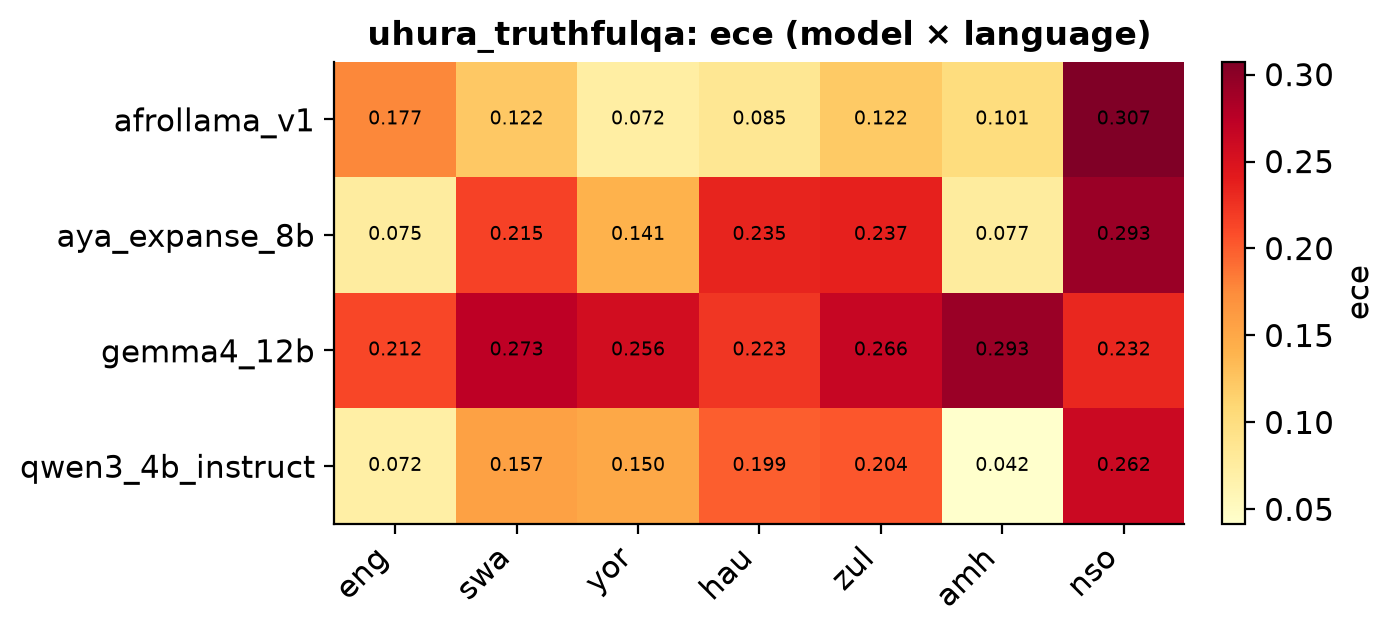
\includegraphics[width=\linewidth]{uhura_ece_heatmap.png}
    \caption{Uhura-TruthfulQA (7 languages)}
  \end{subfigure}\hfill
  \begin{subfigure}{0.49\textwidth}\centering
    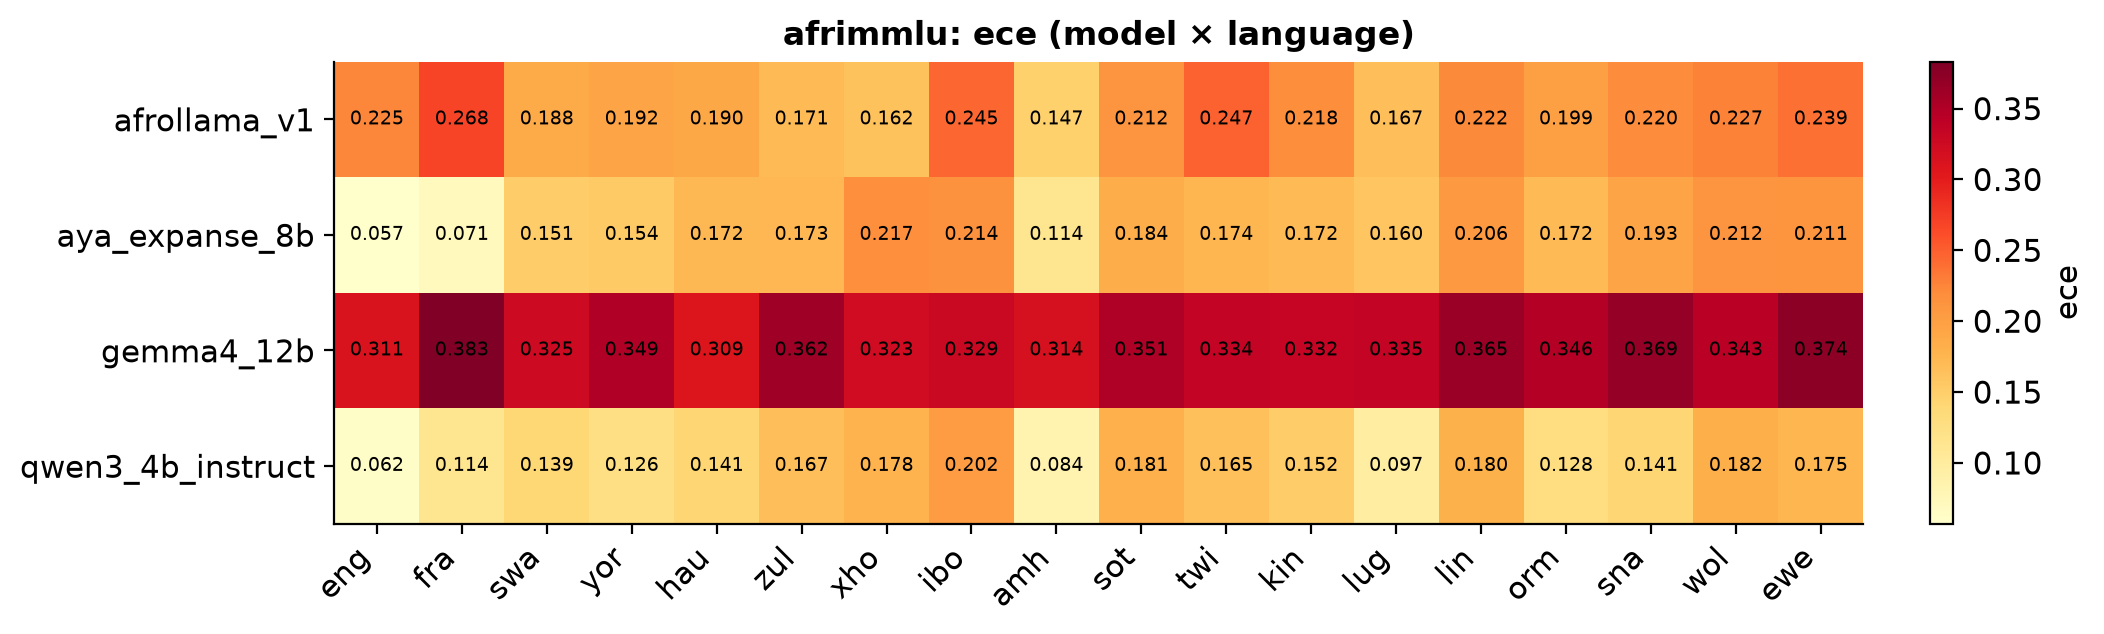
\includegraphics[width=\linewidth]{afrimmlu_ece_heatmap.png}
    \caption{AfriMMLU (18 languages)}
  \end{subfigure}
  \caption{Expected calibration error by model and language. ECE is low in English and French and
  rises across African languages for every model; Gemma is worst throughout.}
  \label{fig:calib}
\end{figure}

\section{Discussion and Limitations}
\textbf{Implications for African AI safety.} In African languages these models are at once less
accurate and more overconfident, the worst combination for trust, since confident wrong answers
reach users precisely where independent verification is hardest. Encouragingly, much of the failure
is an output-layer problem: cheap, post-hoc, per-language temperature scaling closes most of the
calibration gap with no retraining, so safer deployment is feasible now. Abstention alone is
insufficient because the uncertainty signal is weak, so the durable fix remains better
African-language data and training. We distil this into a deployment framework
(Appendix~\ref{app:framework}, Figure~\ref{fig:framework}): recalibrate, then route on calibrated
confidence to answer, request more context, or abstain and defer, logging low-confidence queries to
drive data collection.

\textbf{Limitations.} Accuracies are near chance on these hard, low-resource tasks, so we document
systematic overconfidence rather than catastrophic confident-wrongness, and absolute ECE is moderate
except for Gemma. The weak uncertainty signal (AUROC about 0.55) bounds how much abstention can help.
We cover four open models and two benchmarks; reasoning and frontier closed models were out of scope.
About 15\% of Uhura items lack a recovered topic, so the category analysis uses the labelled subset.

\textbf{Future work.} Reasoning-model and closed-model references; in-context calibration at scale;
the offline data-collection loop in Figure~\ref{fig:framework}; and human-grounded evaluation of
abstention.

\section{Conclusion}
Open LLMs are confidently wrong in African languages, less accurate and more overconfident than in
English, uniformly across four models and two tasks. Post-hoc per-language temperature scaling is a
cheap, effective safety lever that closes most of the calibration gap, and our deployment framework
shows how to combine recalibration with thresholded abstention for safer real-world use.

\noindent\textbf{Code and data.} All code, predictions, figures, and tables are in the repository:
\url{https://github.com/rexsimiloluwah/aims-team-apart-ai-safety-hackathon}. Datasets:
\path{masakhane/uhura-truthfulqa} and \path{masakhane/afrimmlu}.

\noindent\textbf{LLM usage.} We used Claude to help build and debug the evaluation pipeline and to
draft this report; all results were produced by our code and independently verified.

\begin{thebibliography}{9}\small
\bibitem{guo2017} Guo, C., Pleiss, G., Sun, Y., and Weinberger, K. Q. (2017). On Calibration of
Modern Neural Networks. \textit{Proceedings of the 34th International Conference on Machine Learning
(ICML)}, PMLR 70:1321--1330. arXiv:1706.04599.
\bibitem{kuhn2023} Kuhn, L., Gal, Y., and Farquhar, S. (2023). Semantic Uncertainty: Linguistic
Invariances for Uncertainty Estimation in Natural Language Generation. \textit{International
Conference on Learning Representations (ICLR)}. arXiv:2302.09664.
\bibitem{tomani2024} Tomani, C., Chaudhuri, K., Evtimov, I., Cremers, D., and Ibrahim, M. (2024).
Uncertainty-Based Abstention in LLMs Improves Safety and Reduces Hallucinations. arXiv:2404.10960.
\bibitem{uhura} Bayes, E., Azime, I. A., Alabi, J. O., Kgomo, J., Eloundou, T., Proehl, E., Chen, K.,
Khadir, I., Etori, N. A., Muhammad, S. H., Mpanza, C., Thete, I. P., Klakow, D., and Adelani, D. I.
(2024). Uhura: A Benchmark for Evaluating Scientific Question Answering and Truthfulness in
Low-Resource African Languages. arXiv:2412.00948.
\bibitem{irokobench} Adelani, D. I., et al. (2024). IrokoBench: A New Benchmark for African Languages
in the Age of Large Language Models. arXiv:2406.03368.
\bibitem{afrollama} Jacaranda Health (2024). AfroLlama-V1. Hugging Face.
\url{https://huggingface.co/Jacaranda/AfroLlama_V1}.
\end{thebibliography}

\appendix

\section{Models}\label{app:models}
\begin{table}[h]\centering\small
\caption{Open-weight models evaluated. [TEAM: verify AfroLlama parameter count.]}
\label{tab:models}
\resizebox{\textwidth}{!}{%
\begin{tabular}{llll}
\toprule
\textbf{Model} & \textbf{Params} & \textbf{Type} & \textbf{Hugging Face ID}\\
\midrule
Qwen3-4B-Instruct & 4B  & Instruction-tuned & \texttt{Qwen/Qwen3-4B-Instruct-2507}\\
Gemma-4-12B       & 12B & Instruction-tuned & \texttt{google/gemma-4-12B-it}\\
Aya-Expanse-8B    & 8B  & Multilingual      & \texttt{CohereLabs/aya-expanse-8b}\\
AfroLlama-v1      & 8B  & Africa-specific (LLaMA-based) & \texttt{Jacaranda/AfroLlama\_V1}\\
\bottomrule
\end{tabular}}
\end{table}

\section{Metric definitions}\label{app:metrics}
For an item with options $o$ and gold answer $y$, the cloze score of option $o$ with tokens
$o_1,\dots,o_L$ given context $x$ is the length-normalised log-probability
\[
s(o) = \frac{1}{L}\sum_{t=1}^{L}\log p(o_t \mid x, o_{<t}),
\]
\[
p(o) = \operatorname{softmax}_o s(o),
\qquad \hat{y}=\arg\max_o p(o), \qquad c=\max_o p(o).
\]
Over $N$ items with correctness $y_i\in\{0,1\}$, confidence $c_i$, and $B=15$ equal-width confidence
bins $\{B_b\}$:
\[
\mathrm{ECE}=\sum_{b=1}^{B}\frac{|B_b|}{N}\,\bigl|\acc(B_b)-\mathrm{conf}(B_b)\bigr| .
\]
\[
\text{Overconfidence}=\frac{1}{N}\sum_i c_i-\frac{1}{N}\sum_i y_i .
\]
\[
\text{Brier}=\frac{1}{N}\sum_i (c_i-y_i)^2 .
\]
AUROC is the area under the ROC curve using $c$ to rank correct against incorrect items. AUARC is the
area under the accuracy-rejection curve: items are answered most-confident-first and accuracy on the
answered subset is integrated over coverage. Temperature scaling rescales the logits by a single
$T>0$, $p_T(o)=\operatorname{softmax}_o\!\big(s(o)/T\big)$; we fit $T^\star=\arg\min_T \mathrm{ECE}$
on a seeded 50\% calibration split and report ECE on the held-out half.

\section{Prompts}\label{app:scoring}
Each option is scored as a continuation of the prompt; the prompt lists no answer letters.

\begin{tcolorbox}[colback=blue!4,colframe=blue!45,title=\textbf{Uhura-TruthfulQA (truthfulness)},fonttitle=\small,boxrule=0.5pt]
\ttfamily\small Q: \{question\}\\ A:
\end{tcolorbox}

\begin{tcolorbox}[colback=blue!4,colframe=blue!45,title=\textbf{AfriMMLU (knowledge)},fonttitle=\small,boxrule=0.5pt]
\ttfamily\small The following is a multiple-choice question about \{subject\}. Give the correct answer.\\[3pt]
Question: \{question\}\\ Answer:
\end{tcolorbox}

For 5-shot prompting, the prompt is prefixed with five solved examples in the same language, each
formatted as the template above followed by its gold answer text and separated by blank lines; the
examples are held out from evaluation.

\section{Interventions}\label{app:interventions}
\textbf{Temperature scaling.} One temperature $T$ per language, fit by minimising ECE on a seeded
50\% split and evaluated on the other half, searching the grid
\[
T \in \{0.5,\, 0.6,\, 0.7,\, 0.8,\, 0.9,\, 1.0,\, 1.2,\, 1.5,\, 2.0,\, 3.0,\, 5.0\}.
\]
\textbf{Abstention.} The model answers only when confidence $c$ exceeds a per-language threshold
chosen from the risk-coverage curve at a target coverage; we report AUARC over all coverages.
\textbf{Few-shot.} Five in-context examples per language, drawn from held-out items and excluded from
evaluation.

\section{Deployment framework}\label{app:framework}
\begin{figure}[h]\centering
\resizebox{0.92\textwidth}{!}{%
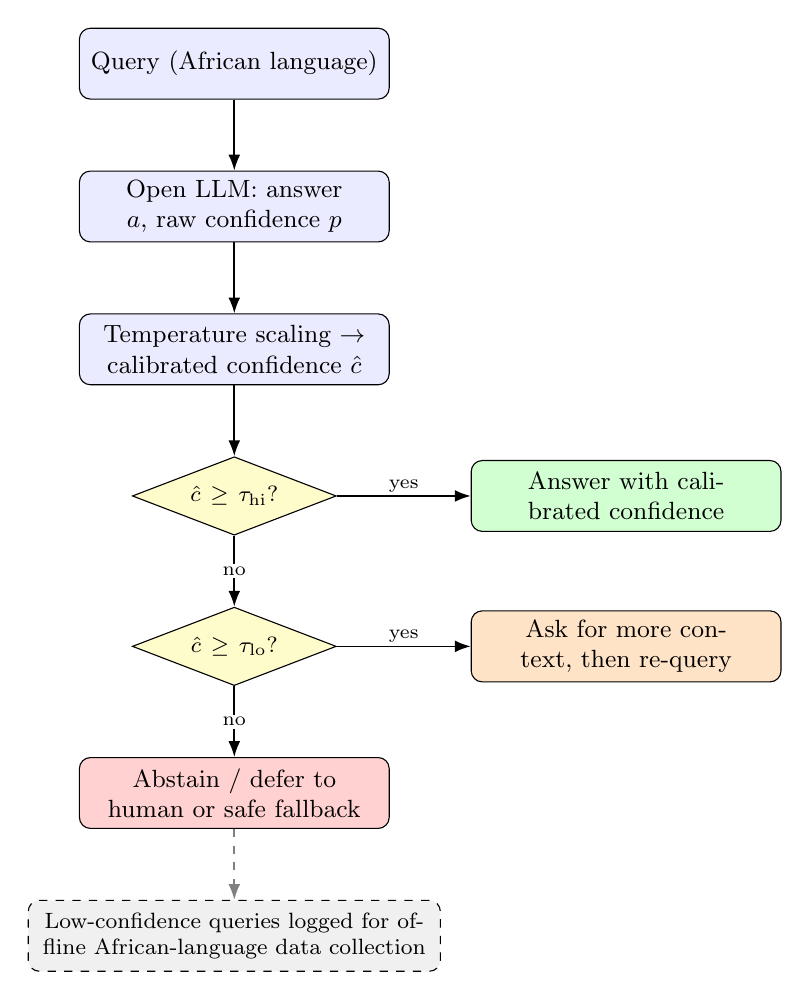
\begin{tikzpicture}[
  node distance=9mm and 17mm,
  box/.style={draw, rounded corners, align=center, text width=37mm, minimum height=9mm, font=\small},
  proc/.style={box, fill=blue!8},
  dec/.style={draw, diamond, aspect=2.6, align=center, fill=yellow!20, font=\footnotesize, inner sep=1pt, text width=17mm},
  good/.style={box, fill=green!18}, warn/.style={box, fill=orange!22}, bad/.style={box, fill=red!18},
  note/.style={box, dashed, fill=gray!12, text width=50mm, font=\footnotesize},
  arr/.style={-{Latex}, semithick}, lbl/.style={font=\scriptsize, fill=white, inner sep=1pt}
]
\node[proc] (q) {Query (African language)};
\node[proc, below=of q] (m) {Open LLM: answer $a$, raw confidence $p$};
\node[proc, below=of m] (ts) {Temperature scaling $\rightarrow$ calibrated confidence $\hat{c}$};
\node[dec, below=of ts] (d1) {$\hat{c}\ge\tau_{\mathrm{hi}}$?};
\node[dec, below=of d1] (d2) {$\hat{c}\ge\tau_{\mathrm{lo}}$?};
\node[bad, below=of d2] (refuse) {Abstain / defer to human or safe fallback};
\node[good, right=of d1] (ans) {Answer with calibrated confidence};
\node[warn, right=of d2] (hedge) {Ask for more context, then re-query};
\node[note, below=of refuse] (log) {Low-confidence queries logged for offline African-language data collection};
\draw[arr] (q)--(m);
\draw[arr] (m)--(ts);
\draw[arr] (ts)--(d1);
\draw[arr] (d1)--(d2) node[lbl,midway]{no};
\draw[arr] (d2)--(refuse) node[lbl,midway]{no};
\draw[arr] (d1)--(ans) node[lbl,midway,above]{yes};
\draw[arr] (d2)--(hedge) node[lbl,midway,above]{yes};
\draw[arr,dashed,gray] (refuse)--(log);
\end{tikzpicture}}
\caption{Deployment framework for LLMs in African languages. Recalibrate first, then route on the
calibrated confidence $\hat{c}$: high values are answered, medium values trigger a request for more
context, and low values are abstained or deferred. Thresholds $\tau$ are set per language from the
risk-coverage curve.}
\label{fig:framework}
\end{figure}

\section{Additional results}\label{app:figs}
Per-dataset figures referenced in the main text. Per-language bootstrap confidence intervals
accompany each per-language table in the repository under \texttt{artifacts/\_comparison/}.

\begin{table}[h]\centering\small
\caption{Zero-shot versus 5-shot on Uhura (values shown as zero-shot $\rightarrow$ 5-shot). Few-shot
gives small gains for three models and backfires on Gemma.}
\label{tab:fewshot}
\begin{tabular}{lccc}
\toprule
\textbf{Model} & \textbf{Accuracy} & \textbf{ECE} & \textbf{Overconfidence}\\
\midrule
Qwen3-4B-Instruct & $0.33 \rightarrow 0.36$ & $0.16 \rightarrow 0.14$ & $0.15 \rightarrow 0.13$\\
AfroLlama-v1      & $0.32 \rightarrow 0.34$ & $0.14 \rightarrow 0.12$ & $0.14 \rightarrow 0.11$\\
Aya-Expanse-8B    & $0.32 \rightarrow 0.33$ & $0.18 \rightarrow 0.17$ & $0.18 \rightarrow 0.16$\\
Gemma-4-12B       & $0.34 \rightarrow 0.31$ & $0.25 \rightarrow 0.33$ & $0.25 \rightarrow 0.33$\\
\bottomrule
\end{tabular}
\end{table}

\begin{figure}[h]\centering
  \begin{subfigure}{0.49\textwidth}\centering
    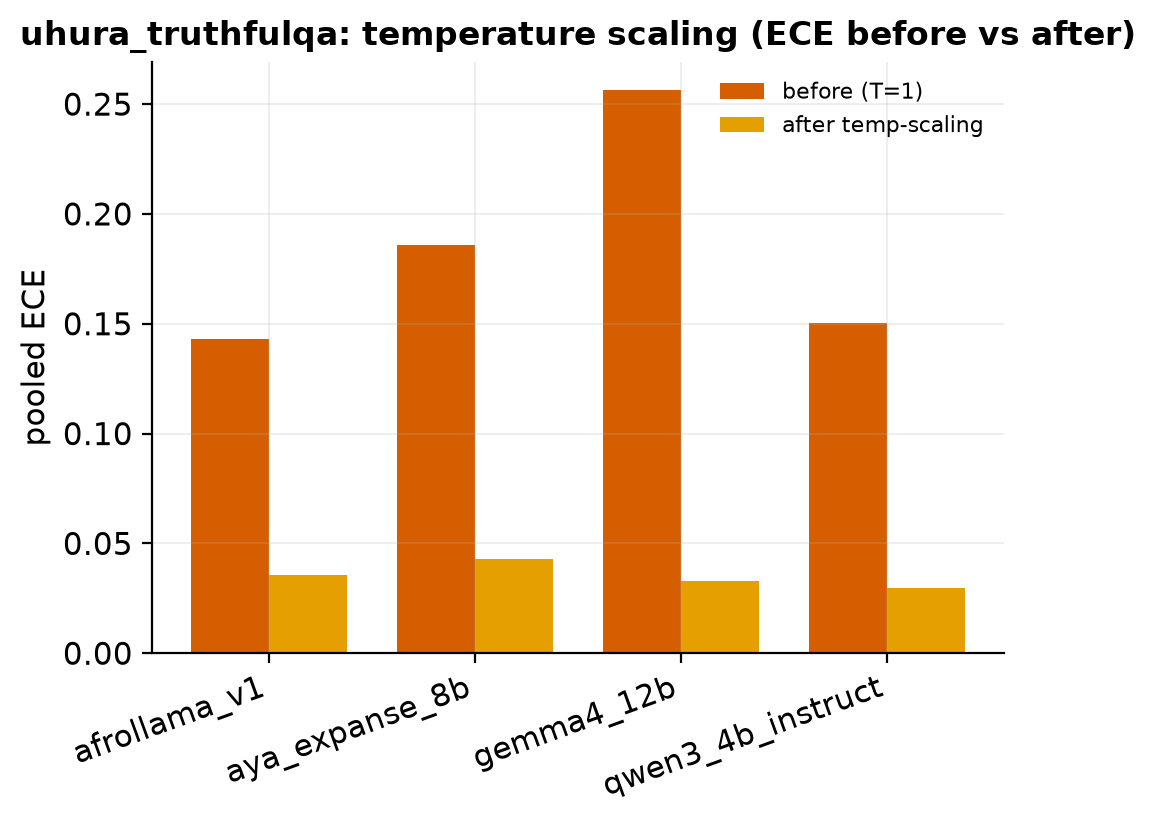
\includegraphics[width=\linewidth]{uhura_temperature_scaling.png}
    \caption{Uhura-TruthfulQA}
  \end{subfigure}\hfill
  \begin{subfigure}{0.49\textwidth}\centering
    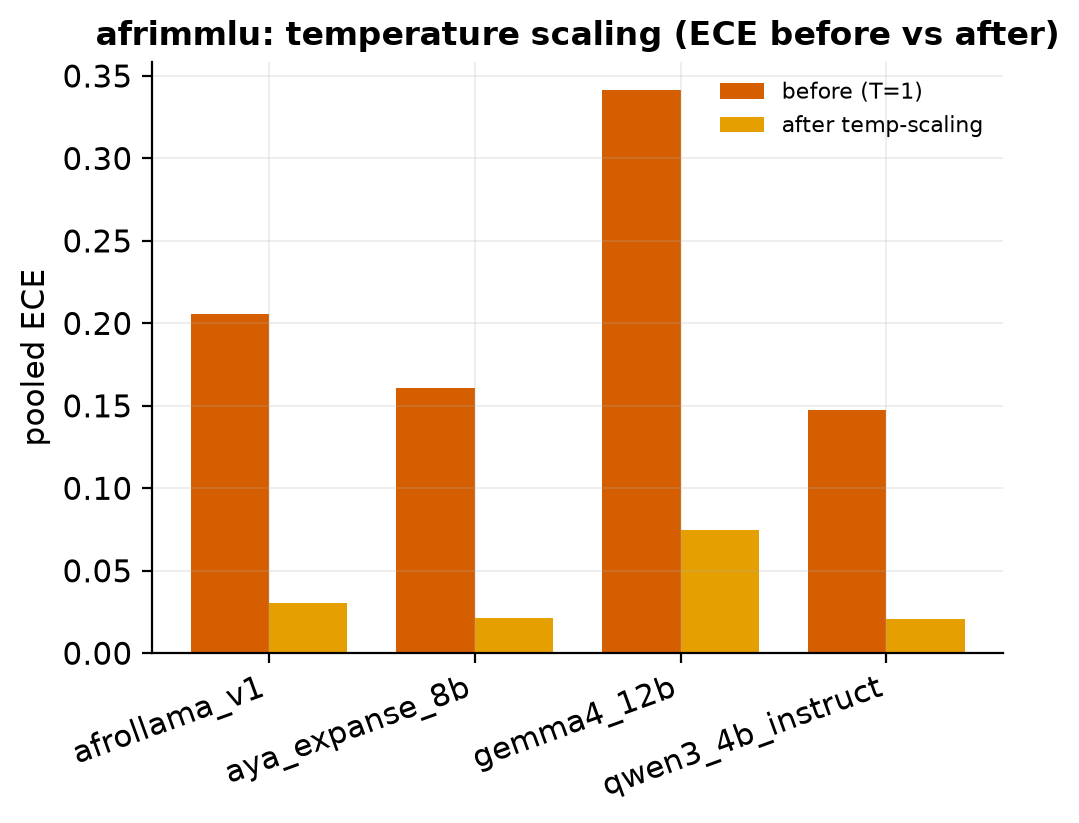
\includegraphics[width=\linewidth]{afrimmlu_temperature_scaling.png}
    \caption{AfriMMLU}
  \end{subfigure}
  \caption{Temperature scaling: pooled ECE before versus after per-language recalibration; ECE drops
  to about 0.03 for all models.}
  \label{fig:tempscale}
\end{figure}

\begin{figure}[h]\centering
  \begin{subfigure}{0.46\textwidth}\centering
    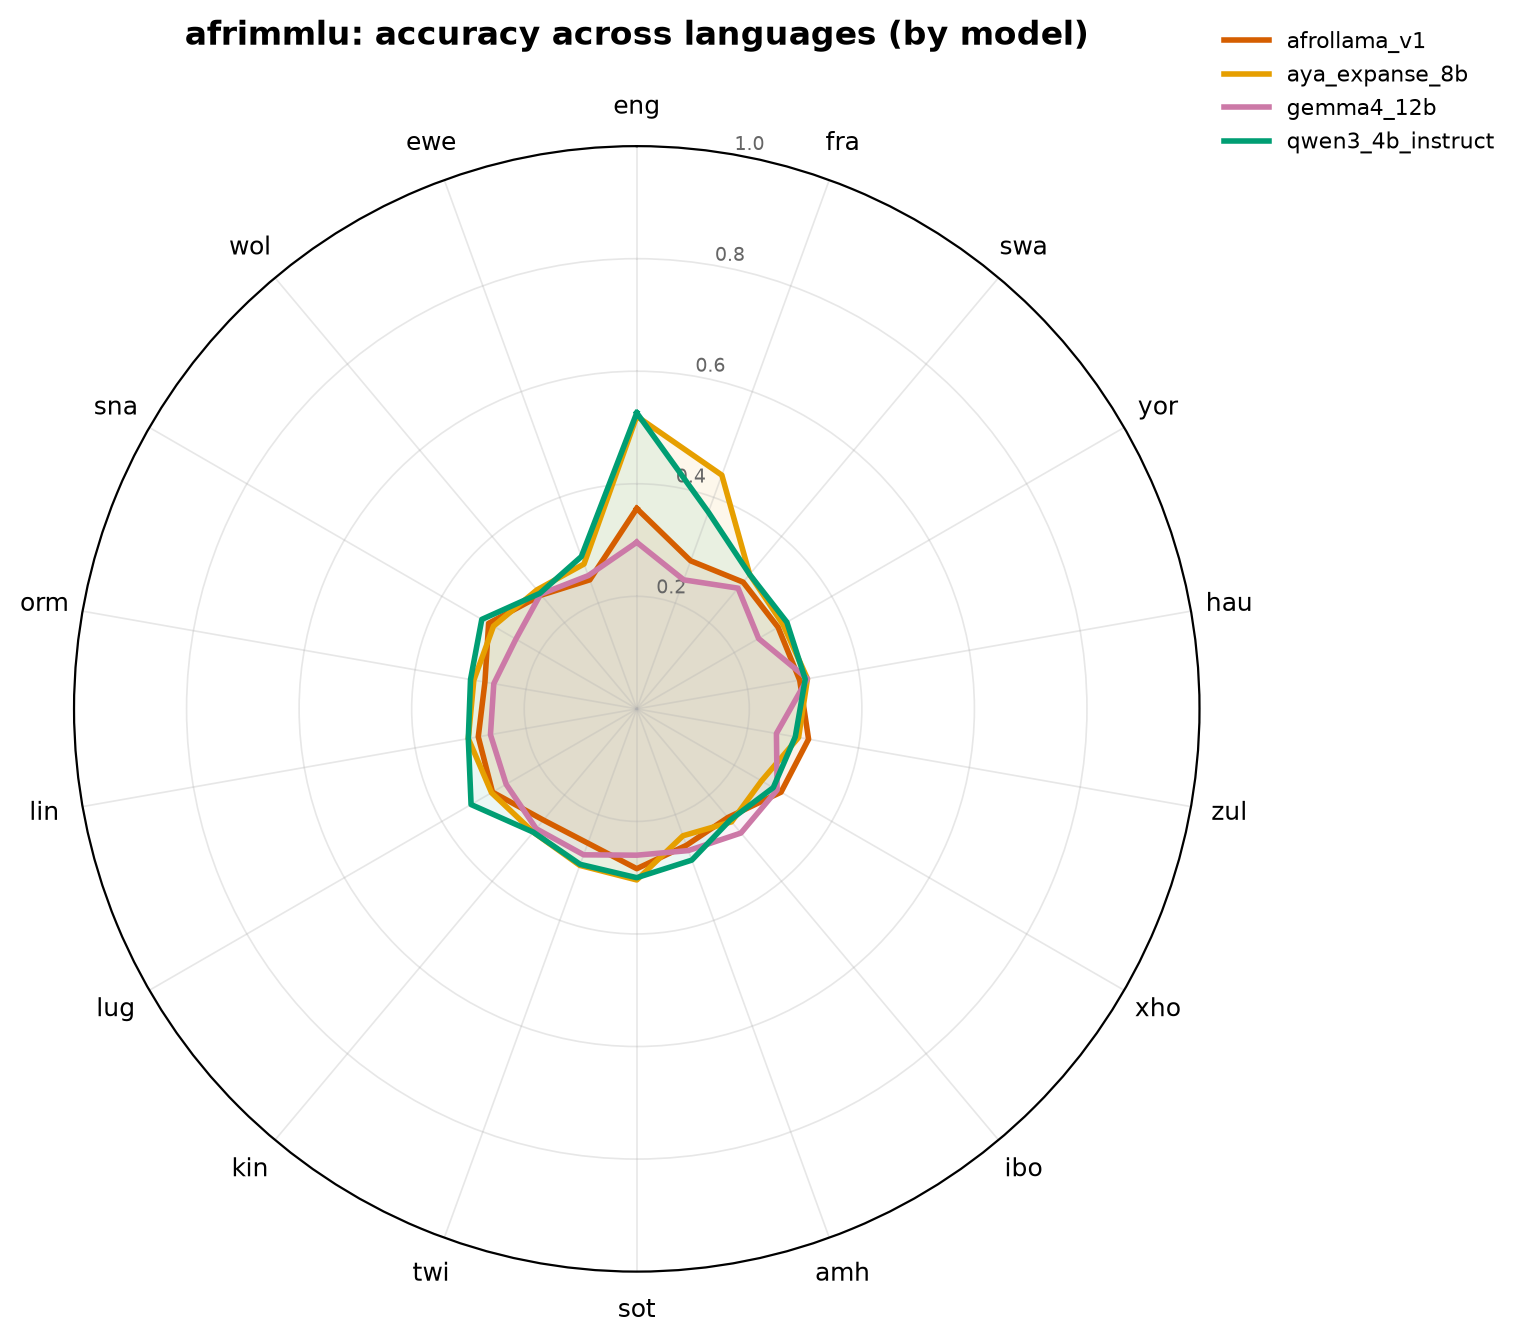
\includegraphics[width=\linewidth]{afrimmlu_accuracy_radar.png}
    \caption{AfriMMLU accuracy by language}
  \end{subfigure}\hfill
  \begin{subfigure}{0.46\textwidth}\centering
    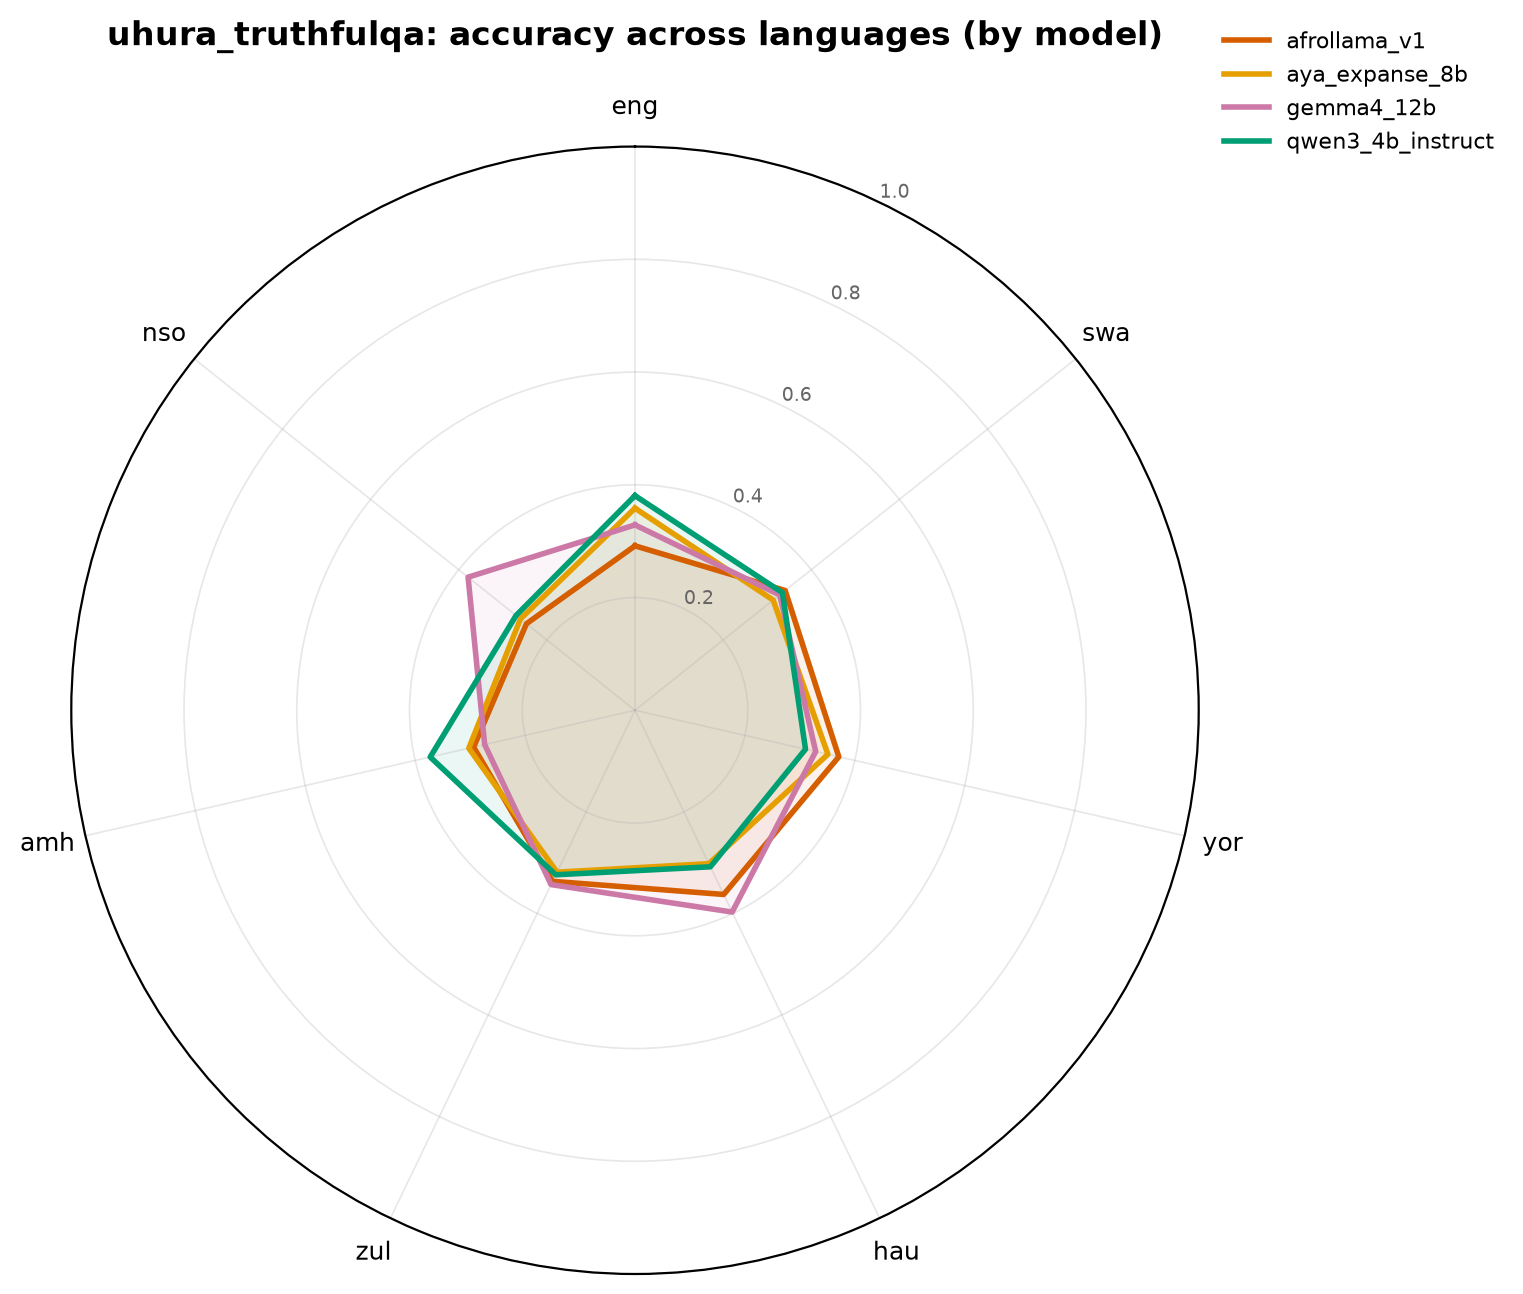
\includegraphics[width=\linewidth]{uhura_accuracy_radar.png}
    \caption{Uhura accuracy by language}
  \end{subfigure}
  \caption{Accuracy across languages by model (factuality decay). Long English and French spokes
  collapse toward chance across African languages.}
  \label{fig:decay}
\end{figure}

\begin{figure}[h]\centering
  \begin{subfigure}{0.46\textwidth}\centering
    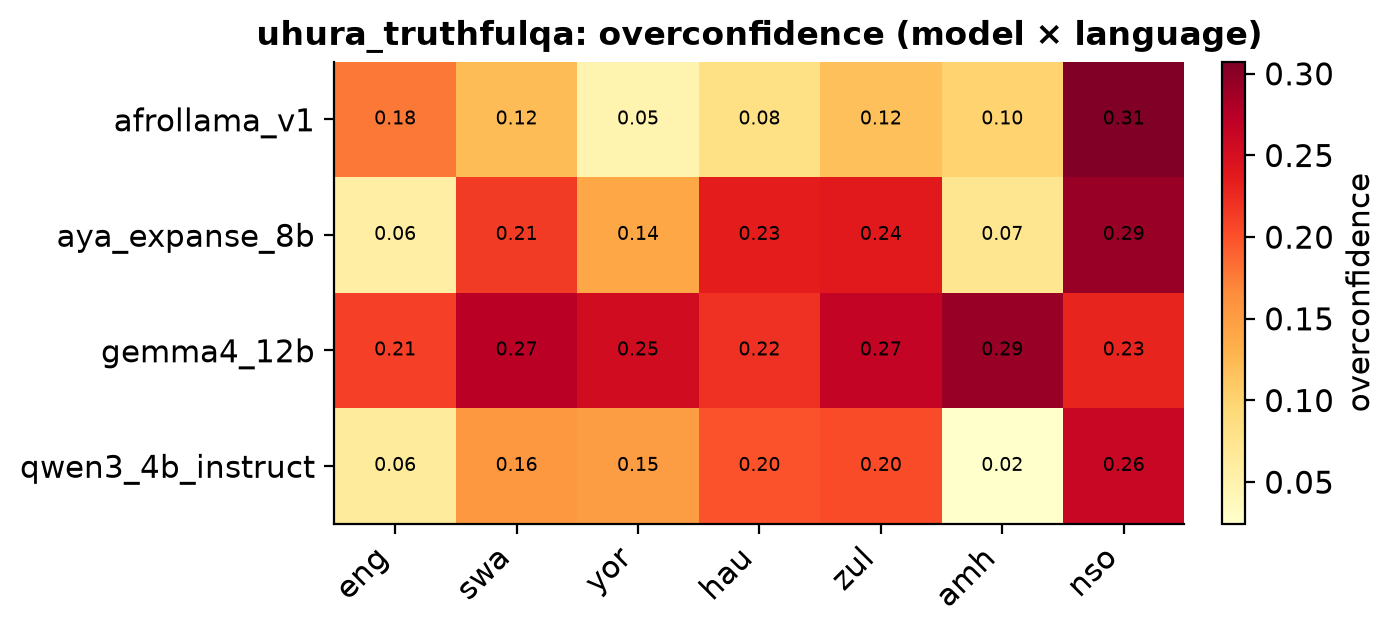
\includegraphics[width=\linewidth]{uhura_overconfidence_heatmap.png}
    \caption{Uhura overconfidence by language}
  \end{subfigure}\hfill
  \begin{subfigure}{0.46\textwidth}\centering
    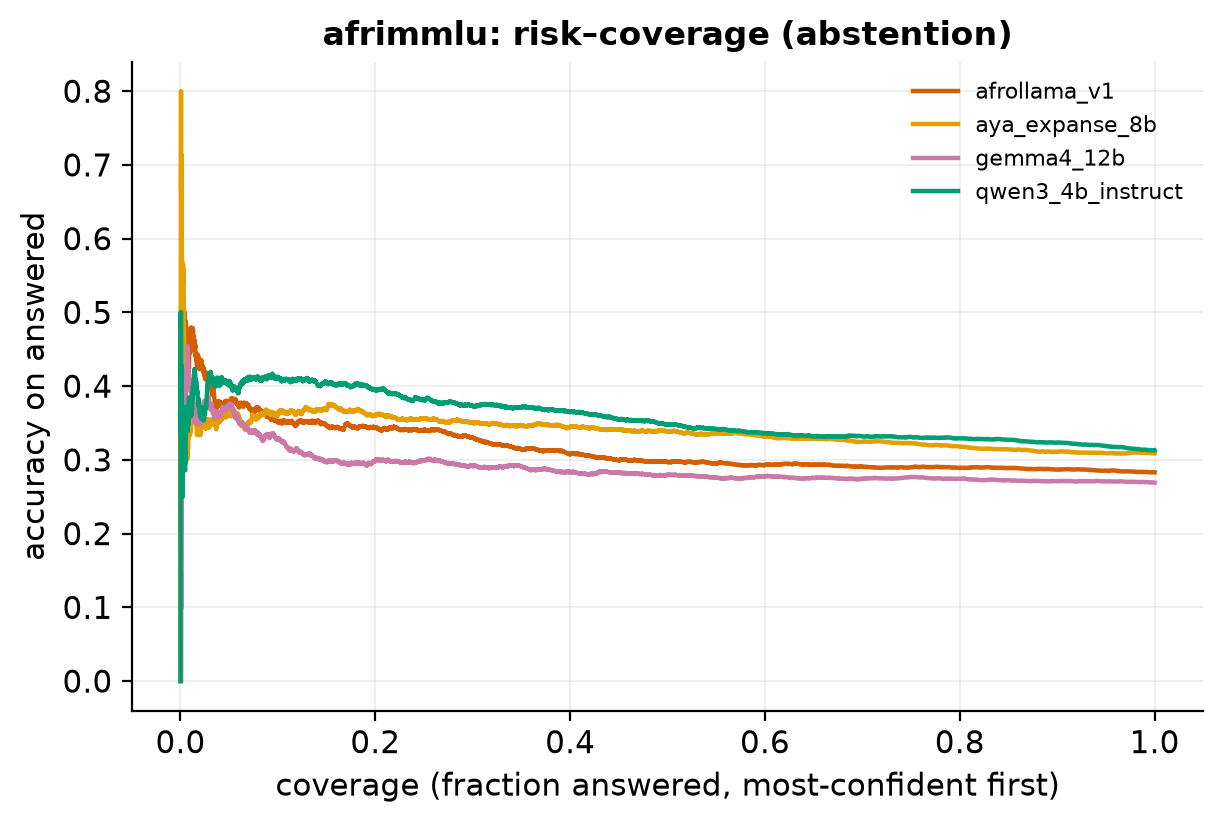
\includegraphics[width=\linewidth]{afrimmlu_risk_coverage.png}
    \caption{AfriMMLU risk-coverage (abstention)}
  \end{subfigure}
  \caption{Overconfidence by language (left) and the accuracy-rejection trade-off under abstention
  (right).}
  \label{fig:appextra}
\end{figure}

\begin{figure}[h]\centering
  \begin{subfigure}{0.46\textwidth}\centering
    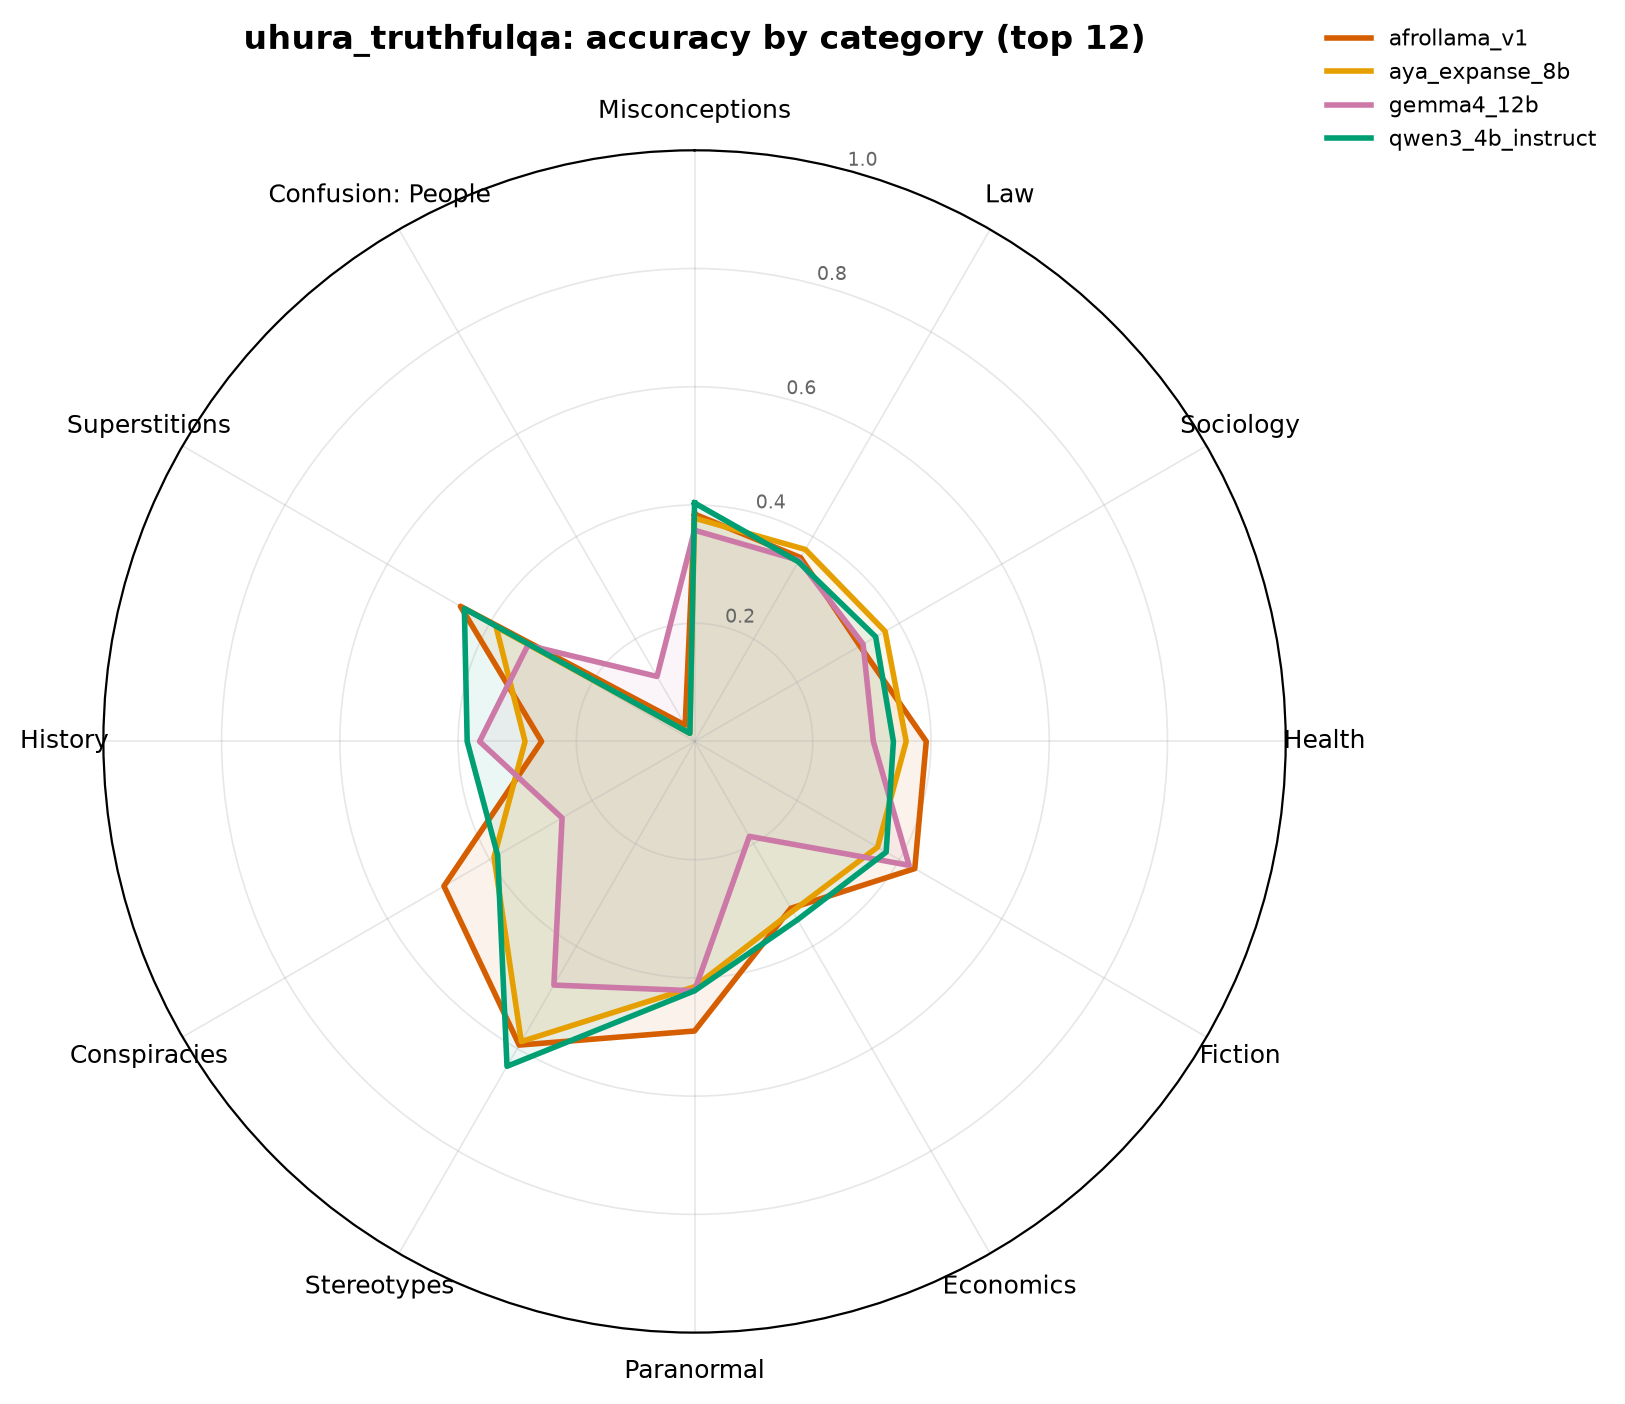
\includegraphics[width=\linewidth]{uhura_category_accuracy_radar.png}
    \caption{Uhura, by topic (top 12)}
  \end{subfigure}\hfill
  \begin{subfigure}{0.46\textwidth}\centering
    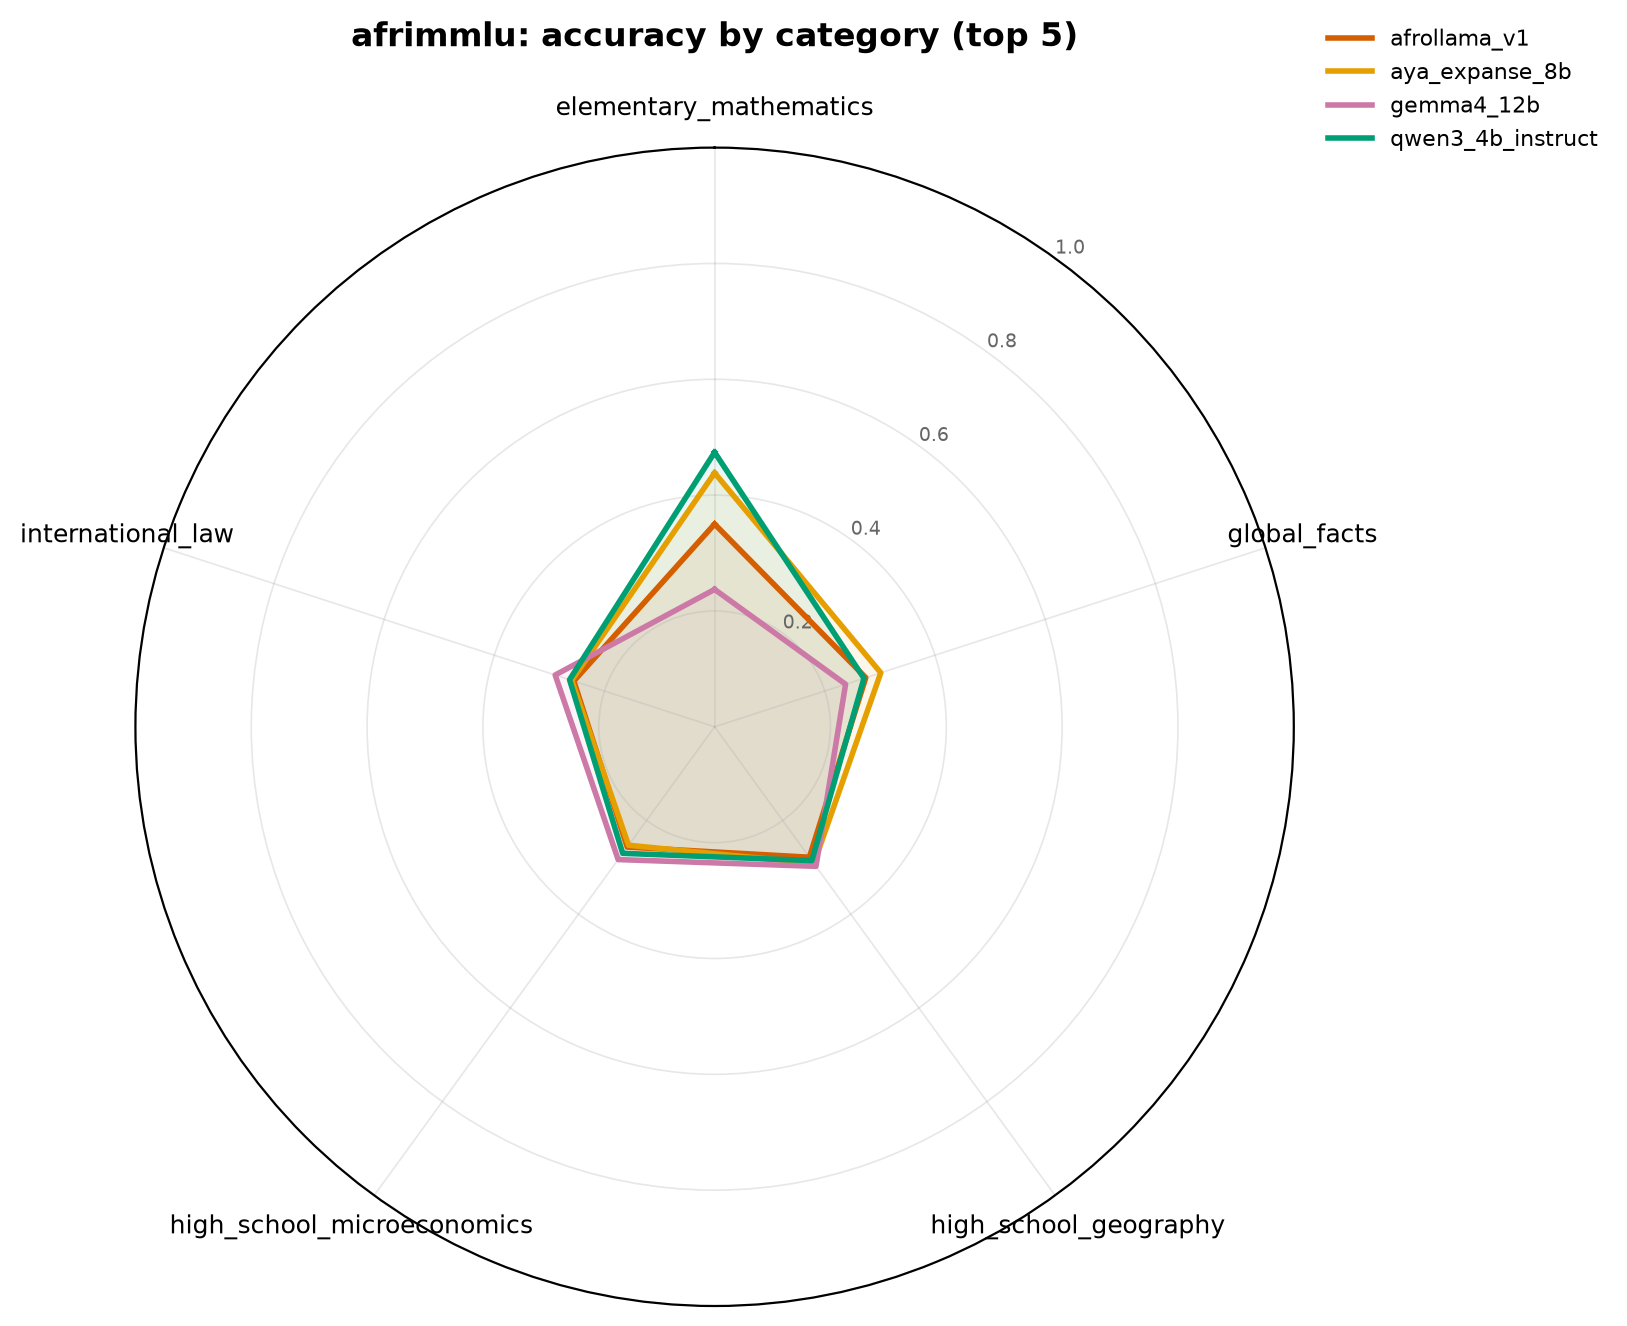
\includegraphics[width=\linewidth]{afrimmlu_category_accuracy_radar.png}
    \caption{AfriMMLU, by subject}
  \end{subfigure}
  \caption{Accuracy across question categories by model.}
  \label{fig:appcat}
\end{figure}

\end{document}
